\documentclass[11pt]{amsart}

\usepackage[T1]{fontenc}
\usepackage[utf8]{inputenc}
\usepackage{lmodern}
\input{glyphtounicode}
\pdfgentounicode=1

\usepackage{amsmath,amssymb}
\usepackage{array,booktabs,tabularx}
\usepackage{graphicx}
\usepackage{geometry}
\usepackage{xcolor}
\usepackage{enumitem}
\usepackage{placeins}
\usepackage{hyperref}
\geometry{margin=1in}
\setlength{\emergencystretch}{3em}
\graphicspath{{figures/}}
\hypersetup{
  colorlinks=true,
  linkcolor=blue!45!black,
  citecolor=blue!45!black,
  urlcolor=blue!45!black,
  pdftitle={Supplementary Numerical Results for Projected Multilinear Models},
  pdfauthor={Eliuth Chavero Jasso}
}

\newcommand{\norm}[1]{\lVert#1\rVert}

\title{Supplementary Numerical Results\\ for Projected Multilinear Models}
\author{Eliuth Chavero Jasso}
\address{Independent Researcher, Apizaco, Tlaxcala, Mexico}
\thanks{Supplement to \cite{ChaveroJassoNumerical}. Every figure is regenerated from the
committed experiment records by \texttt{generate\_figures.py}; the mapping from figure to
input file, with checksums, is in \texttt{figure\_provenance.json}.}
\date{31 July 2026}

\begin{document}
\maketitle

\begin{abstract}
Nine figures supporting the numerical study \cite{ChaveroJassoNumerical}, together with the
information needed to regenerate each of them: the generating script, the input files, the
parameters, and checksums of inputs and outputs. Each figure is supplied as a vector PDF,
an archival SVG and a raster PNG at 300 dots per inch, from a single generator run.
Captions state whether a displayed quantity is an analytical bound, an identity holding by
construction, or an observed value, and every logarithmic axis with a plotting floor states
that floor. Section~\ref{sec:sources} lists the data sources, Section~\ref{sec:params} the
parameters of each experiment, and Section~\ref{sec:notincluded} the material that is
deliberately not included.
\end{abstract}

\section{Figures}
\label{sec:figures}

\begin{figure}[htbp]
\centering
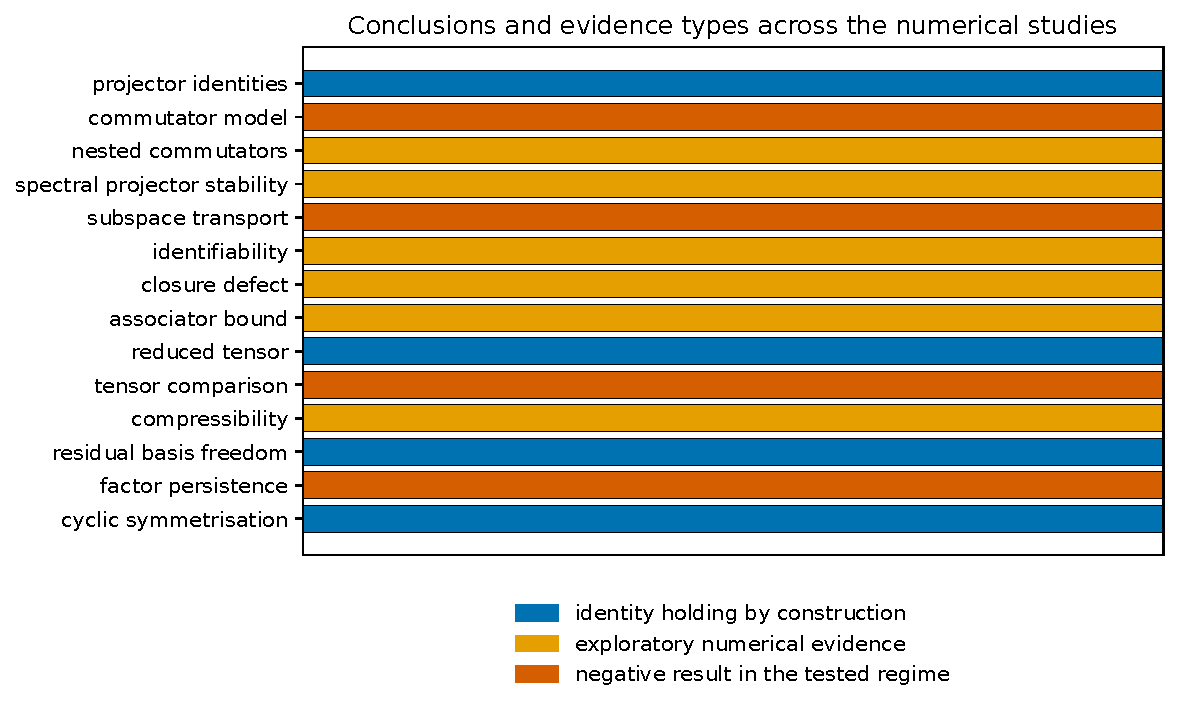
\includegraphics[width=0.82\textwidth]{01_evidence_summary}
\caption{Summary of conclusions and evidence types across the numerical studies. Each of
the fourteen experiments of \cite{ChaveroJassoNumerical} is classified into exactly one of
three categories: an identity holding by construction, exploratory numerical evidence, or a
negative result in the tested regime. The classification is editorial and follows the
scheme stated in that article; no experiment contributes to a combined score, and none is
ranked against another.}
\label{fig:summary}
\end{figure}

\begin{figure}[htbp]
\centering
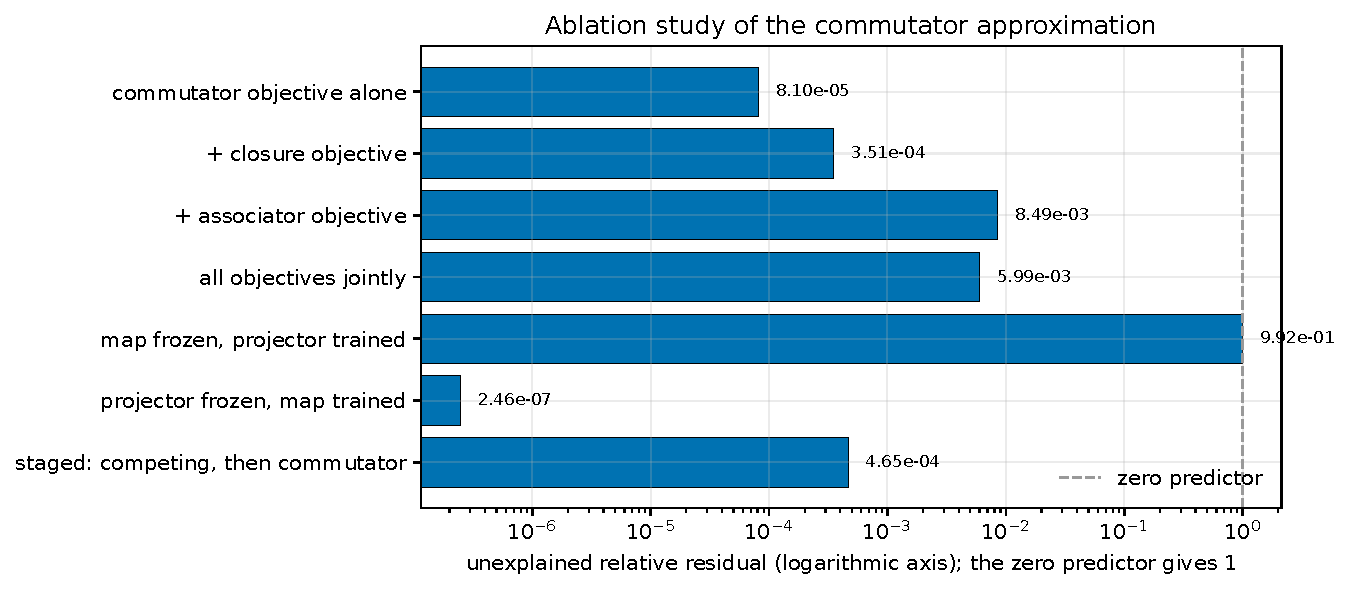
\includegraphics[width=0.88\textwidth]{02_commutator_ablation}
\caption{Ablation study of the commutator approximation. Seven training regimes, one run
each, at ambient dimension $16$, reduced rank $4$, representation rank $4$ and $400$
optimisation steps. The horizontal axis is the unexplained relative residual on a
logarithmic scale; the dashed line marks the zero predictor, which gives the value $1$.
Every bar is drawn at the value recorded in the experiment file and none is displayed at a
plotting floor; in particular the regime with the projector frozen reaches
$2.46\times10^{-7}$, which is the numerical floor of that run and not zero. Freezing the
map and training only the projector leaves the residual at $0.9925$; freezing the projector
and training only the map, with the projector left at its random initial value, reaches the
smallest residual of the seven. One run per regime: this is exploratory evidence, not a
replicated experiment.}
\label{fig:ablation}
\end{figure}

\begin{figure}[htbp]
\centering
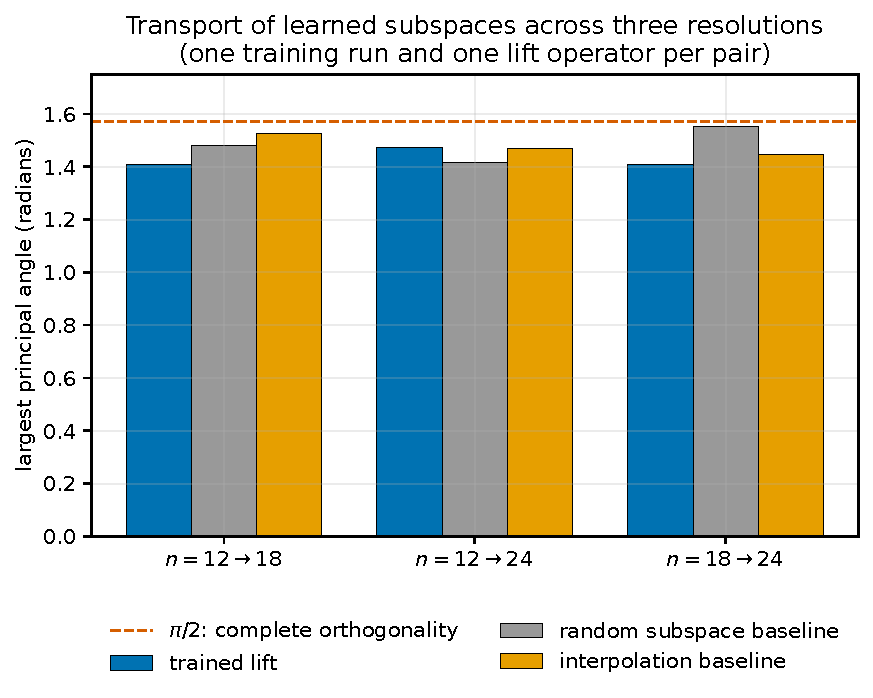
\includegraphics[width=0.78\textwidth]{03_subspace_transport}
\caption{Transport of learned subspaces across three independently trained resolutions.
For each ordered resolution pair, the largest principal angle between the transported
subspace and the independently learned subspace, for the trained lift and for two
baselines. The dashed line is $\pi/2\approx1.571$ radians, complete orthogonality. All
quantities lie between $1.407$ and $1.553$ radians. The trained lift improves on both
baselines in two of the three pairs, by $0.02$ to $0.15$ radians, which is small relative
to how close every condition already is to complete orthogonality. One training run and one
lift operator per pair; no uncertainty interval is available and none is drawn.}
\label{fig:transport}
\end{figure}

\begin{figure}[htbp]
\centering
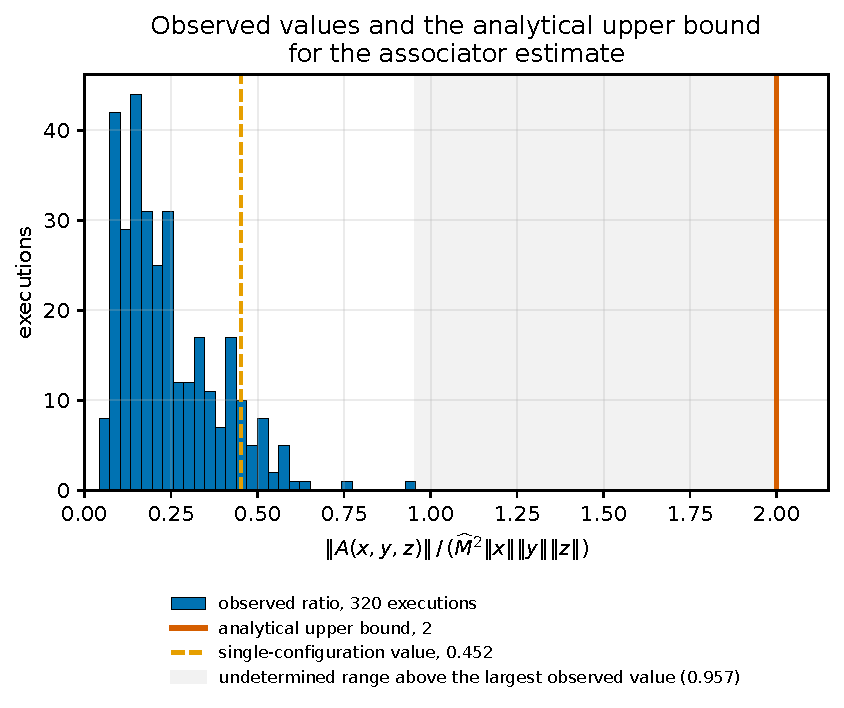
\includegraphics[width=0.76\textwidth]{04_associator_bound}
\caption{Observed values and the analytical upper bound for the associator estimate.
Histogram of the observed ratio $\norm{A(x,y,z)}/(\widehat M^{2}\norm{x}\norm{y}\norm{z})$
over the $320$ executions of the broad sweep. The solid vertical line is the triangle bound
of value $2$, which is an analytical upper bound and not an observation. The dashed line is
the single-configuration value $0.452$ reported in \cite{ChaveroJassoNumerical}. The shaded
band is the range between the largest observed value and the bound, in which the exact
constant is undetermined; it is not an uncertainty interval.}
\label{fig:associator}
\end{figure}

\begin{figure}[htbp]
\centering
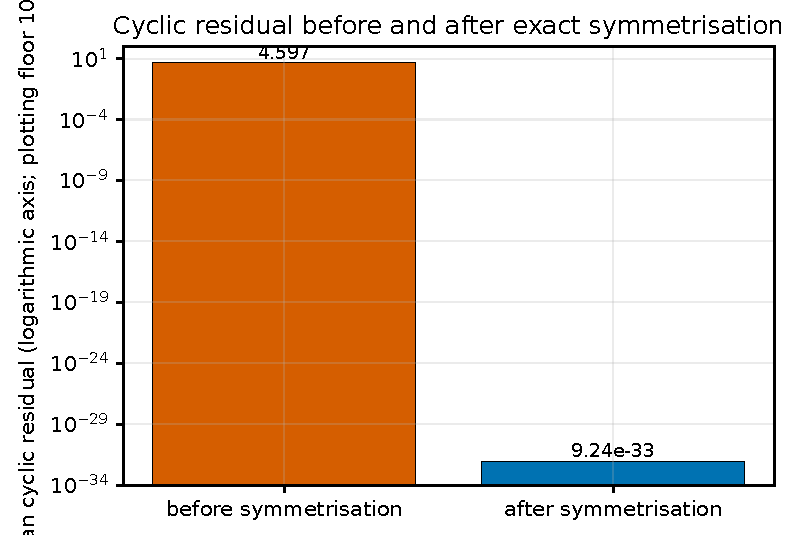
\includegraphics[width=0.66\textwidth]{05_cyclic_symmetrisation}
\caption{Cyclic residual before and after exact symmetrisation, on a logarithmic axis with
plotting floor $10^{-34}$, as stated on the axis. The value after symmetrisation is at the
numerical floor \emph{by construction}: cyclic averaging is an orthogonal projector onto the
cyclically invariant subspace, so its output is cyclic identically. The figure confirms
that the implementation applies that projector correctly. It is not evidence that a
symmetry was learned.}
\label{fig:cyclic}
\end{figure}

\begin{figure}[htbp]
\centering
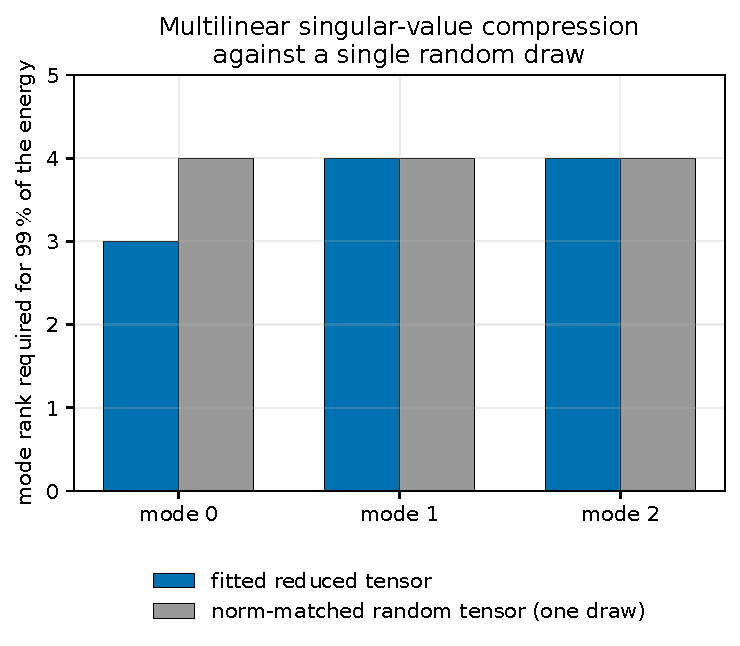
\includegraphics[width=0.66\textwidth]{06_compression}
\caption{Multilinear singular-value compression against a single random draw. Mode ranks
required to capture $99\,\%$ of the energy, for a fitted reduced tensor and for one
norm-matched random tensor, at a single configuration. The fitted tensor is more
compressible in one of the three modes and equally compressible in the other two. One
random draw is a control, not a null distribution, and no distributional statement follows
from this figure.}
\label{fig:compression}
\end{figure}

\begin{figure}[htbp]
\centering
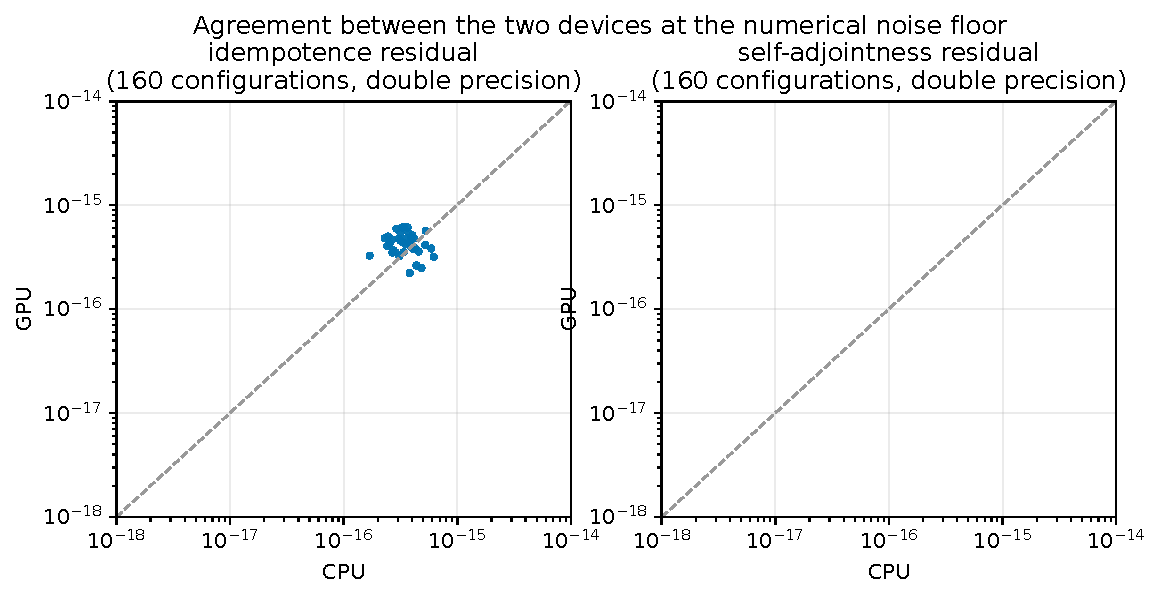
\includegraphics[width=0.94\textwidth]{07_device_agreement}
\caption{Agreement between the two devices at the numerical noise floor. Each point is one
configuration, with its CPU value on the horizontal axis and its GPU value on the vertical
axis, in double precision with reduced-precision matrix multiplication disabled; the dashed
line is equality. Both residuals lie at the noise floor on both devices, so the figure
shows agreement of the implementation, not accuracy of any quantity of interest. Values
below $10^{-20}$ are drawn at that floor.}
\label{fig:agreement}
\end{figure}

\begin{figure}[htbp]
\centering
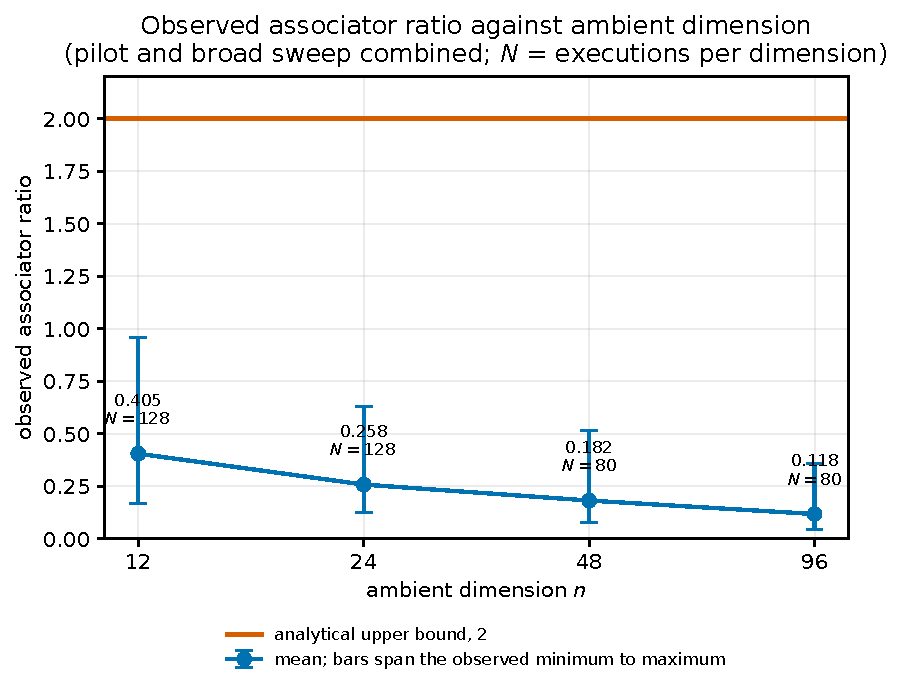
\includegraphics[width=0.80\textwidth]{08_associator_vs_dimension}
\caption{Observed associator ratio against ambient dimension, over the pilot and broad
sweeps combined. Markers are means and bars span the observed minimum to maximum; the
number of executions contributing to each point is annotated. The mean decreases
monotonically from $0.405$ at $n=12$ to $0.118$ at $n=96$, moving further from the
analytical bound of $2$ as the ambient dimension grows, not closer. The
single-configuration value $0.452$ of Figure~\ref{fig:associator}, measured at $n=16$, is
consistent with this trend. The bars are observed ranges, not confidence intervals. The two
executions of a configuration, one per device, are not independent observations; the counts
shown are executions.}
\label{fig:trend}
\end{figure}

\begin{figure}[htbp]
\centering
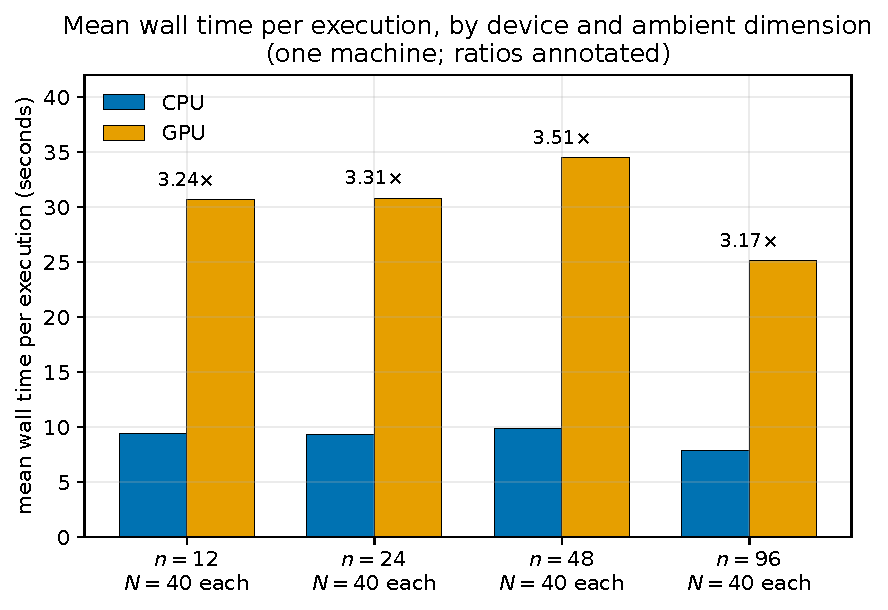
\includegraphics[width=0.80\textwidth]{09_device_throughput}
\caption{Mean wall time per execution, by device and ambient dimension, over the $160$
configurations of the broad sweep, with $40$ executions per device per dimension. The
annotated ratios are between $3.17$ and $3.51$ and show no trend towards crossover across
an eightfold range in ambient dimension. This is a measurement on one machine and one
software stack; it supports no asymptotic-complexity statement and no comparison between
hardware platforms.}
\label{fig:throughput}
\end{figure}

\FloatBarrier

\section{Data sources and provenance}
\label{sec:sources}

Every figure is produced by \texttt{generate\_figures.py} from files in \texttt{data/},
which are verbatim copies of the committed experiment records. The generator writes
\texttt{figure\_provenance.json}, containing for each figure: the input files with their
SHA-256 checksums and sizes; the output files in all three formats with their SHA-256
checksums and sizes; the SHA-256 of the generator itself; and the versions of the numerical
libraries used. No value in any figure is entered by hand.

\begin{table}[h]
\centering\small
\caption{Input file for each figure.}
\label{tab:sources}
\begin{tabularx}{\linewidth}{@{}lX@{}}
\toprule
Figure & Input \\
\midrule
\ref{fig:summary} & classification stated in \cite{ChaveroJassoNumerical}; no data file \\
\ref{fig:ablation} & \texttt{data/block\_b\_ablation\_matrix.json} \\
\ref{fig:transport} & \texttt{data/block\_e\_interscale\_experiment.json} \\
\ref{fig:associator} & \texttt{data/s1\_results.parquet} \\
\ref{fig:cyclic} & \texttt{data/s1\_results.parquet} \\
\ref{fig:compression} & mode ranks at the reference configuration, stated in \cite{ChaveroJassoNumerical} \\
\ref{fig:agreement} & \texttt{data/s1\_results.parquet} \\
\ref{fig:trend} & \texttt{data/pilot\_results.parquet}, \texttt{data/s1\_results.parquet} \\
\ref{fig:throughput} & \texttt{data/s1\_results.parquet} \\
\bottomrule
\end{tabularx}
\end{table}

\section{Parameters of the swept experiments}
\label{sec:params}

\begin{table}[h]
\centering\small
\caption{Design of the two sweep stages. A configuration is one distinct mathematical
setting; an execution is one run of a configuration on one device. Each configuration was
executed once on the CPU and once on the GPU, so the two executions of a configuration are
not independent observations.}
\label{tab:design}
\begin{tabularx}{\linewidth}{@{}lrrX@{}}
\toprule
stage & configurations & executions & grid \\
\midrule
pilot & $48$ & $96$ & arity $\in\{3,4\}$, $n\in\{12,24\}$, rank $\in\{3,6\}$,
representation rank $\in\{4,8\}$, $3$ seeds \\
broad & $160$ & $320$ & as above, with $n\in\{12,24,48,96\}$ and $5$ seeds \\
\midrule
total & $208$ & $416$ & \\
\bottomrule
\end{tabularx}
\end{table}

There were no failures in either stage. Summed over the per-execution records, wall time was
$942.8$ seconds for the pilot and $6300.8$ seconds for the broad stage. Both stages ran in
double precision with reduced-precision matrix multiplication explicitly disabled and
deterministic algorithms enabled; the hardware is described in \cite{ChaveroJassoSoftware}.

\section{Visual conventions}
\label{sec:conventions}

\begin{itemize}[leftmargin=*]
\item The palette is Okabe--Ito, which is colourblind-safe; no encoding relies on
distinguishing red from green.
\item Every figure is produced as a vector PDF, which is what the manuscript includes; SVG
and 300-dpi PNG versions are supplied alongside.
\item Where a logarithmic axis cannot display a value, the plotting floor is stated on the
axis and the true value is annotated.
\item Where a figure shows a range, the caption states whether it is an observed
minimum--maximum range or something else. No confidence interval is drawn anywhere in this
supplement, because no sampling model is specified for any of these experiments.
\item Sample counts are given on the figure or in its caption.
\item Optimiser restarts and repeated executions of the same configuration are never used
as replicates.
\end{itemize}

\section{What is deliberately not included}
\label{sec:notincluded}

The following material is absent, and is listed rather than silently omitted.

\begin{itemize}[leftmargin=*]
\item Figures relating to the finite-dimensional theory of projected composition trees
--- topology, dimension and $\eta$ dependence, and the geometry of the coefficients $k$ and
$k-1$. These belong to \cite{ChaveroJassoTrees} and appear there.
\item A full diagram of the residual basis freedom, beyond the single degenerate-eigenspace
example described in \cite{ChaveroJassoNumerical}, and an atlas of the permutations and
signs of the generalised Jacobi expression. The underlying data exist but were not turned
into figures.
\item Adversarial maxima of the closure defect across a swept grid. Figure~\ref{fig:trend}
provides the analogous surface for the associator; the closure defect was not swept.
\item Device agreement for the ten experiments that were not extended over the grid. Those
were run on the CPU only, so no comparison is possible.
\item Any figure aggregating the fourteen experiments into a single score. No such score is
formed anywhere in this work.
\end{itemize}

\bibliographystyle{amsplain}
\bibliography{references}

\end{document}
